\section{Sistema experto}
En este apartado se tratarán los pasos que se tienen que seguir para desarrollar un sistema experto.
 En la fitura 3.1 se puede ver cual es el ciclo de vida para la creación y mantenimiento de un software
 como el mencionado anteriormente.
%En este apartado se abordarán los pasos a seguir para desarrollar un sistema experto.
 %En la figura 3.1 se puede observar el ciclo de vida de creación y mantenimiento de un software
 %de este tipo:

\begin{figure}[htb]
  \centering
    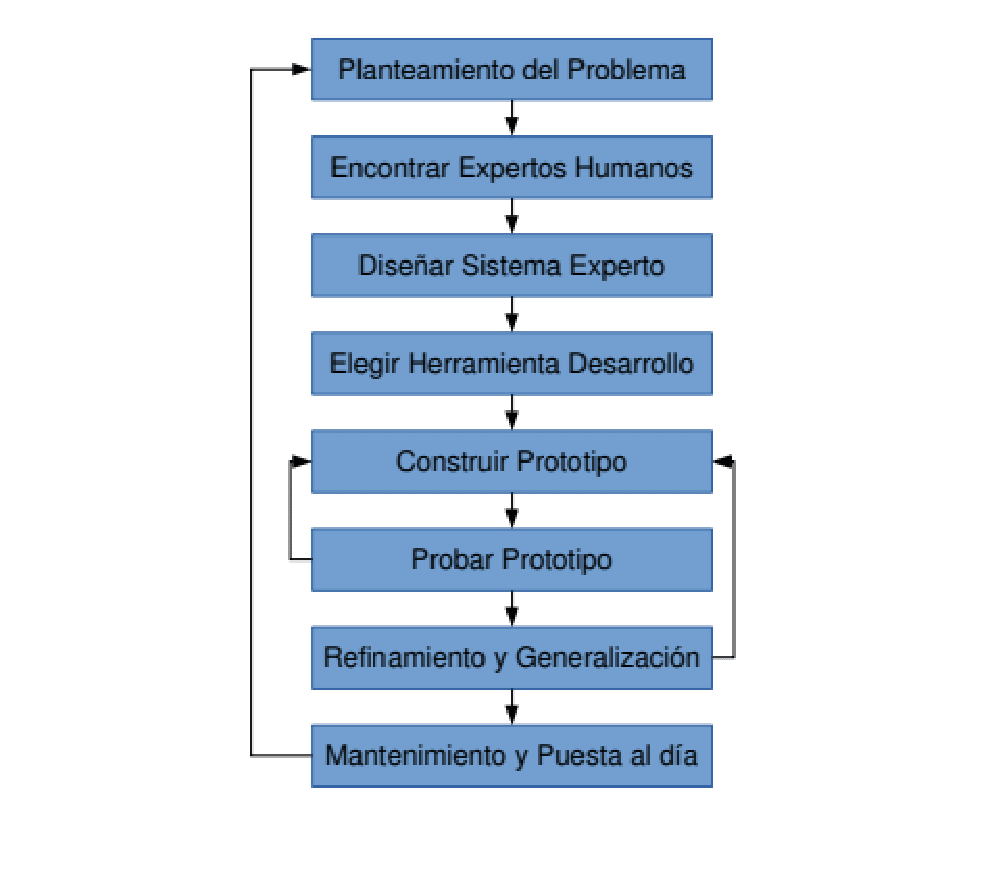
\includegraphics[width=0.4\linewidth]{DesarrolloSE}
  \caption[Desarrollo SE]{Desarrollo SE}
  \label{fig:Desarrollo Sistema Experto}
\end{figure}

A continuación se enumeran los pasos específicos para la creación del sistema experto.
\begin{enumerate}
  \item Características del sistema experto
  \item Estudio de viabilidad
  \item Adquisición del conocimiento
  \item Implantación
  \item Evaluación y pruebas
\end{enumerate}

\subsection{Características del sistema experto}
%inicio pendiente de revision palabras

Ante la situación de querer desarrollar un sistema experto lo primero que se tendrá
 que hacer será definir el alcance y los límites de dicho sistema. Esto quiere decir que
 habrá que indicar que cubre y que no nuestro sistema experto. De esta forma sabremos
 cuales son sus limitaciones y en un futuro que se podrá ampliar.

%Cuando se desea implementar un sistema experto en primer lugar se debe definir el
 %alcance y los límites de dicho sistema, se deben indicar que aspectos cubre el
 %sistema experto y que aspectos quedan fuera del ámbito del sistema.

Aquí se definirán las características del problema al que nos enfrentamos.
 La intención de este apartado es conocer cuál es la naturaleza del problema
 y que objetivos se pretenden cumplir de manera que se sepa como va a ayudar
 nuestro sistema experto a la solución de dichos problemas. Para ello habrá
 una interacción entre el ingeniero de conocimiento y el experto. El experto
 será quien enseñe al ingeniero una serie de casos y será este último el que se
 encargue de desarrollar un primer enfoque del problema. Dentro de estas interacciones
 serán las mas comunes que el ingeniero le muestre el conocimiento adquirido
 y el experto le ayude a refinar y aclarar los posibles errores. De esta manera
 y con las iteraciones que sean necesarias se acabará llegando a una descripción
 lo mas real posible.

%Define las características del problema. Se pretende determinar la naturaleza
 %del problema y los objetivos precisos que indique exactamente cómo se espera
 %que el sistema experto contribuya a la solución de los problemas. Existirá
 %una interacción entre experto e ingeniero. Cuando el experto en el dominio
 %muestre distintos casos, el ingeniero del conocimiento desarrolla una primera descripción
 %del problema. Normalmente el experto no esta de acuerdo con ella, o mejor dicho,
 %no siente que representa el problema en su totalidad, entonces el ingeniero reformulará
 %la descripción. Esta actividad prosigue hasta que los dos estén de acuerdo en la
 %descripción.

%fin pendiente de revision palabras

\subsection{Estudio de viabilidad}
%inicio pendiente de revision palabras

Una vez que se ha definido el alcance del sistema experto deberá hacerse un estudio
 previo a la implementación para conocer la viabilidad de este sistema desde un punto
 de vista computacional. Para ello se hará un estudio de viabilidad. En este caso se
 utilizará el test de SLAGEL. Este estudio establecerá si el proyecto cumple con las
 estas características:

%Teniendo claro el alcance del sistema experto debe estudiarse si la implementación
 %del mismo es posible desde el punto de vista de la computación. Para esto se
 %realiza un estudio de viabilidad, en este caso se utiliza un estudio de viabilidad basado
 %en el test de SLAGEL. Este estudio establece sie l proyecto cumple con las siguientes
 %características.

\begin{compactitem}
  \item \textbf{Plausible}: Determina si es posible resolver el problema desde el
     punto de vista de la ingeniería del conocimiento.
  \item \textbf{Justificable}: Analiza si está justificado el desarrollo del
     sistema desde la perspectiva de la ingeniería dle conocimiento, se basa en
     temas como la necesidad del sistema y la inversión a realizar.
  \item \textbf{Adecuado}: Establece si el problema a resolver está dentro
     del marco de la ingeniería del conocimiento, existen problemas que son más
     adecuados resolverlos por métodos tradicionales.
  \item \textbf{Éxito}: Determina las probabilidades de éxito del sistema a
     desarrollar, es una estimación
\end{compactitem}

El método del test de SLAGEL se define en el Anexo A.
%fin pendiente de revision palabras


\subsection{Adquisición del conocimiento}
%inicio pendiente de revision palabras


Uno de los pilares y por lo general con mayor complejidad a la hora de implementar
 un sistema experto es obtener el conocimiento, el cual suele ser a través de un experto,
 para después volcarlo en el sistema experto. Para ello hay muchos métodos y herramientas
 entre las cuales se encuentran la entrevista, observación y creación de escenarios.

%Una de las partes más importantes y a la vez más complicadas de la implementación
 %de un sistema experto es obtener el conocimiento, normalmente un experto, y
 %volcarlo en el sistema experto. Existen muchas herramientas y métodos para obtener
 %este conocimiento entre las cuales está la entrevista, la observación y la creación
 %de escenarios.

La adquisición del conocimiento trata de que las personas que no son expertas en la materia
 donde se va a implementar el sistema experto, obtengan el conocimiento necesario para ser
 capaces de resolver problemas de diferentes fuentes. El proceso de obtención del conocimiento
 sigue varias etapas las cuales se resumen en las siguientes:
%La adquisición del conocimiento es la principal complicación en el desarrollo de
 %Sistemas Expertos. Consiste en que las personas no expertas en el dominio donde
 %se va a desarrollar el Sistema Experto extraigan el conocimiento necesario para resolver
 %problemas de diversas fuentes. El proceso de adquisición del conocimiento ha seguido
 %diferentes etapas que podrían resumirse en las siguientes:

\begin{compactitem}
  \item Primeras reuniones con los expertos y evaluación de la viabilidad del proyecto.
  \item Extración de conocimientos, a partir de la documentación disponible, como
     por ejemplo libros, conferencias, internet, etc.
  \item Deducción de conocimientos a partir de los expertos.
\end{compactitem}

Además se logra la familiarización del Ingeniero del Conocimiento en el contexto en
 el que se va a trabajar. Se busca en las primeras reuniones describir conocimientos
 generales, así como afianzarse con la terminología.

La estructura de las entrevistas junto a casos de entrevistas se define en el anexo B.

Después de obtener el conocimiento será definir unas estructuras para poder organizarlo.
 Será en esta etapa donde el ingeniero del conocimiento decide que estructuras serán
 las mas adecuadas para este sistema experto, eso si, previamente tiene que estar perfectamente
 definido el problema en toda su magnitud, sin haber hecho referencia a técnicas de programación
 o solo habiendo tenido en cuenta métodos exitosos en IA. Con estructura adecuada se hace referencia
 aquella que da una solución total o parcial al problema analizado previamente. Una de las
 diferentes responsabilidades del ingeniero de conocimiento será analizar situaciones tipo y
 a partir de ellas extraer las reglas que serán las que describan el conocimiento del experto
 en la materia.

%Una vez obtenido el conocimiento hay que designar estructuras para organizar el
 %el conocimiento. Después de haber determinado el problema en toda su magnitud,
 %sin haberse referido a técnicas de programación o a indagar solo en los métodos
 %que son exitosos en inteligencia artificial, es en esta etapa donde el ingeniero del
 %conocimiento selecciona las estructuras apropiadas a este sistema experto en particular.
 %Es decir, que dan solución total o parcial al problema analizado en las etapas precedentes.
 %Una de las responsabilidades principales del ingeniero del conocimiento es analizar
 %situaciones tipo y a partir de ellas extraer las reglas que describen el conocimiento del
 %experto en el dominio.

%fin pendiente de revision palabras

\subsection{Implantación}
%inicio pendiente de revision palabras

Desarrolla la transformación de los conocimientos representados en el modelo formal
 en un modelo computable.

Será en esta etapa en la que se elaboren las reglas que lleven el conocimiento adquirido
 previamente. Se utilizarán las herramientas y técnicas predeterminadas para implementar
 un prototipo del sistema. Este prototipo será utilizado para probar y evaluar los avances
 que se hacen en el proyecto. Se volverá a etapas anteriores en caso de que el resultado
 no sea satisfacotrio para poder perfeccionarlo. Cuando haya alcanzado un grado optimo
 de satisfacción como para poder ser ejecutado, el sistema experto estará listo para ser probado.

%Elaboración de las reglas que incorporen el conocimiento. Se peretende en esta ocasión
 %usar las herramientas y técnicas predeterminadas para implementar una primera versión
 %o prototipo del sistema. Este prototipo esta destinado a evaluar los progresos que se
 %van haciendo, y por ende, retornar a etapas anteriores si es necesario.

%Una vez que el sistema prototipo se ha perfeccionado lo suficiente para ser ejecutado,
 %el sistema experto estará listo para ser probado.

%fin pendiente de revision palabras

\subsection{Evaluación y pruebas}
%inicio pendiente de revision palabras

En esta fase se establece el grado de experiencia que adquirió el sistema. Cualquier
 experto en la materia, hayan o no participado en el proyecto, se comprometen a evaluar
 la capacidad del sistema. Estos expertos trataran de entrever la calidad de dicho sistema
 asistiendo en diferentes casos de problemas que tendrá que resolver el software. Otra de
 las cosas que tendránque evaluar será la amplitud que posee el repositorio de casos y como
 el sistema experto guía su uso.

%Establece el grado de experiencia alcanzado por el sistema. De manera tal que expertos
 %en el área que han o no partilcipado en el desarrollo del proyecto se comprometen a
 %evaluar el desempeño del sistema, tratando de vislumbrar la calidad de asistencia que
 %brinda el Sistema Experto ante diferentes casos de problemas a resolver por software.
 %También se evalúa la amplitud y generalidad de marcos compuestos que posee el repositorio
 %y cómo el sistema guía su uso.

Una vez el sistema sea capaz de llevar a cabo el mismo trabajo que haría un especialista
 podremos decir que está preparado.


%Se considera que el sistema experto está terminado cuando realiza trabajos a nivel
 %del especialista. Entonces, el proceso de prueba no esta listo hasta que las soluciones
 %propuestas por el sistema seantan válidas como las propuestas por el experto humano.
%fin pendiente de revision palabras

\subsection{Motor de inferencia}
%inicio pendiente de revision palabras
El sistema experto que se va a desarrollar siguiendo la metodología anterior va
 a funcionar sobre un motor de inferencia desarrollado para tal fin, el motor
 de inferencia se basa en el motor implementado para CLIPS y a continuación se van
 a detallar las características de dicho motor.

\subsubsection{Algoritmo de selección de reglas aplicables en CLIPS}
\begin{compactitem}
  \item Elegir la regla aplicable con máxima prioridad.
  \item Elegir la regla según estrategia de resolución de conflictos.
  \item Elegir de forma arbitraria.
\end{compactitem}

Estas son las estrategias definidas en el motor de inferencia de CLIPS para
 la selección de reglas aplicables o activas son varias:

\begin{compactitem}
  \item \textbf{Depth Strategy (estrategia por defecto)}. Una activación que contiene el hecho
    más reciente se sitúa por encima de las activaciones con igual o mayor antigüedad.
 \item \textbf{Breadth Strategy}. Una activación que contiene el hecho más reciente se
    sitúa por debajo de las activaciones con igual o mayor antigüedad.
 \item \textbf{Complexity Strategy}. Las nuevas activaciones se sitúan por encima de las
    activaciones con igual o menor especificidad (no de comparaciones que han de
    realizarse en el antecedente una la regla).
 \item \textbf{Simplicity Strategy}. Las nuevas activaciones se sitúan por debajo de las
    activaciones con igual o mayor especificidad.
 \item \textbf{LEX Strategy}. Se ordenan los time-tag en orden decreciente y se comparan
    uno a uno, hasta encontrar uno mayor que otro, en caso de que no haya el mismo
    número de time-tag se añaden ceros al final.
 \item \textbf{MEA Strategy}. Parecido a LEX, pero mirando sólo el primer patrón que
    equipara en la regla.
 \item \textbf{Random Strategy}. A cada activación se le asigna un número aleatorio para
    determinar su orden en la agenda.
\end{compactitem}

\subsubsection{Definición de prioridades en CLIPS}
\begin{compactitem}
  \item Asignar un valor de prioridad (entero positivo) a cada regla.
  \item En CLIPS se definen como propiedades de reglas.
  \item Se recomienda minimizar el uso de prioridades de reglas.
\end{compactitem}

%fin pendiente de revision palabras
